\documentclass[border=6pt]{standalone}
\usepackage{pgfplots}
\pgfplotsset{compat=1.18}
\usepackage{xcolor}
\definecolor{s0}{HTML}{2A78D6}
\definecolor{s1}{HTML}{86B6EF}
\definecolor{s2}{HTML}{A8420C}
\definecolor{s3}{HTML}{DD6B33}
\definecolor{s4}{HTML}{EE9A6A}
\definecolor{surface}{HTML}{FCFCFB}
\definecolor{ink}{HTML}{0B0B0B}
\definecolor{muted}{HTML}{52514E}
\definecolor{gridc}{HTML}{E8E7E3}
\begin{document}
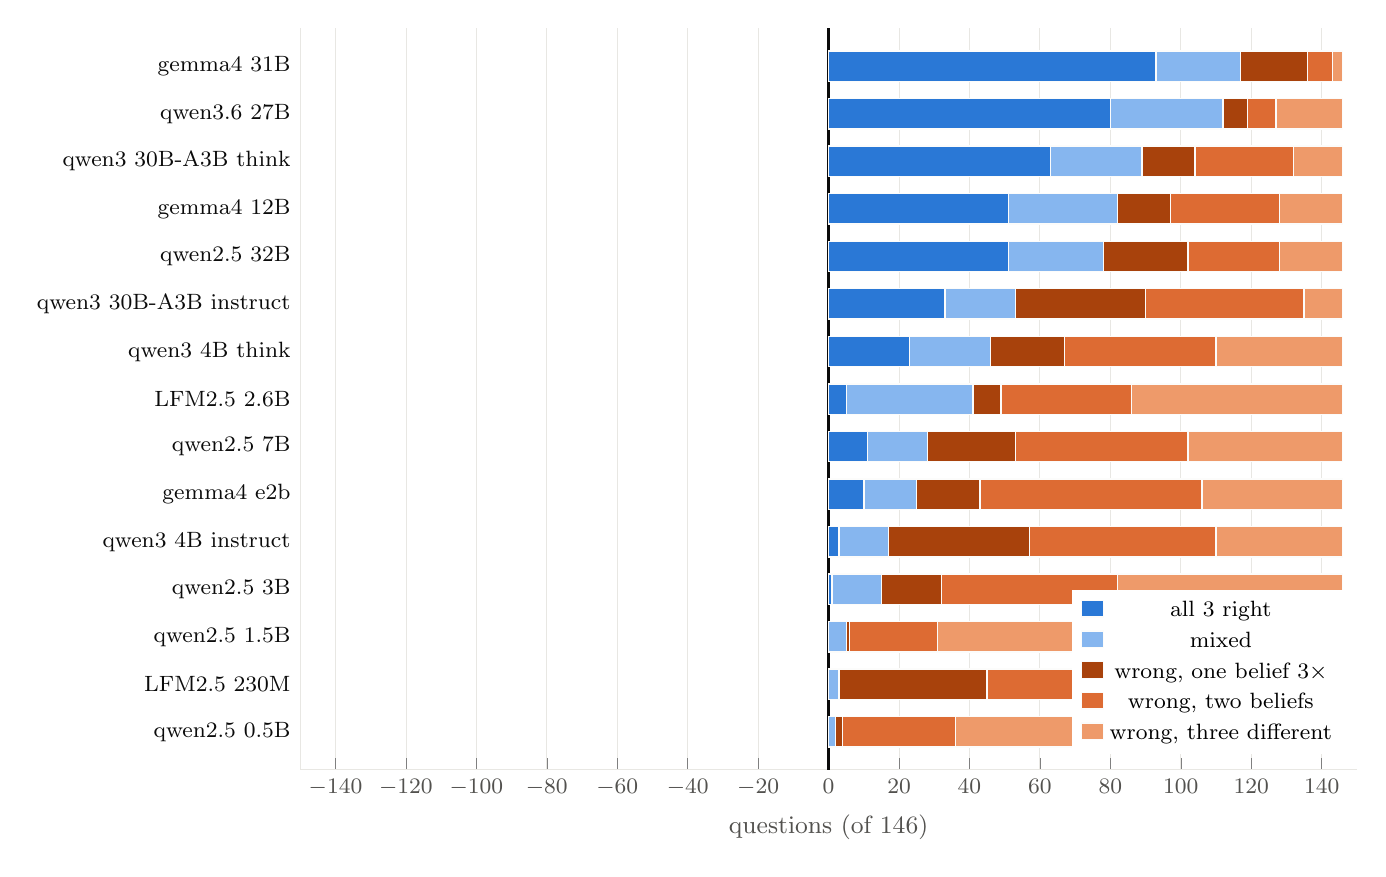
\begin{tikzpicture}
\begin{axis}[
  width=15cm, height=11cm,
  xbar stacked, bar width=11pt,
  xmin=-150, xmax=150, ymin=-0.8, ymax=14.8,
  xlabel={questions (of 146)},
  xlabel style={font=\small, color=muted},
  tick label style={font=\footnotesize, color=muted},
  ytick={0,1,2,3,4,5,6,7,8,9,10,11,12,13,14},
  yticklabels={gemma4 31B,qwen3.6 27B,qwen3 30B-A3B think,gemma4 12B,qwen2.5 32B,qwen3 30B-A3B instruct,qwen3 4B think,LFM2.5 2.6B,qwen2.5 7B,gemma4 e2b,qwen3 4B instruct,qwen2.5 3B,qwen2.5 1.5B,LFM2.5 230M,qwen2.5 0.5B},
  y dir=reverse, ytick style={draw=none},
  yticklabel style={font=\footnotesize, color=ink},
  xmajorgrids, grid style={gridc, line width=0.3pt},
  axis line style={gridc}, axis x line*=bottom, axis y line*=left,
  legend style={draw=none, font=\footnotesize, at={(0.99,0.02)}, anchor=south east, legend columns=1},
  x filter/.code={\pgfmathparse{abs(\pgfmathresult)}},
]
\addplot[fill=s0, draw=surface, line width=0.5pt] coordinates {(-93,0) (-80,1) (-63,2) (-51,3) (-51,4) (-33,5) (-23,6) (-5,7) (-11,8) (-10,9) (-3,10) (-1,11) (0,12) (0,13) (0,14)};
\addlegendentry{all 3 right}
\addplot[fill=s1, draw=surface, line width=0.5pt] coordinates {(-24,0) (-32,1) (-26,2) (-31,3) (-27,4) (-20,5) (-23,6) (-36,7) (-17,8) (-15,9) (-14,10) (-14,11) (-5,12) (-3,13) (-2,14)};
\addlegendentry{mixed}
\addplot[fill=s2, draw=surface, line width=0.5pt] coordinates {(19,0) (7,1) (15,2) (15,3) (24,4) (37,5) (21,6) (8,7) (25,8) (18,9) (40,10) (17,11) (1,12) (42,13) (2,14)};
\addlegendentry{wrong, one belief 3$\times$}
\addplot[fill=s3, draw=surface, line width=0.5pt] coordinates {(7,0) (8,1) (28,2) (31,3) (26,4) (45,5) (43,6) (37,7) (49,8) (63,9) (53,10) (50,11) (25,12) (58,13) (32,14)};
\addlegendentry{wrong, two beliefs}
\addplot[fill=s4, draw=surface, line width=0.5pt] coordinates {(3,0) (19,1) (14,2) (18,3) (18,4) (11,5) (36,6) (60,7) (44,8) (40,9) (36,10) (64,11) (115,12) (43,13) (110,14)};
\addlegendentry{wrong, three different}
\draw[ink, line width=1pt] (axis cs:0,-0.8) -- (axis cs:0,14.8);
\end{axis}
\end{tikzpicture}
\end{document}
